\chapter{프리드만 팽창, 복사, 암흑 물질}

\section{기본 우주론 방정식 복습}

은하단보다 큰 규모에서는 우주가 균일하다고 가정한다. 좌표를 정해 우리가 \(x=0\)에 있고, 대표적인 은하 하나, 또는 허블 흐름을 따라 움직이는 가상의 입자 하나가 \(x=1\)에 있다고 하자. 정의에 따라 그 입자와 우리 사이의 물리적 거리는 척도 인자 \(a(t)\)이다. \(x=2\)에 있는 점까지의 거리는 \(2a(t)\)이고, 나머지도 마찬가지다.

\begin{figure}[ht]
\centering
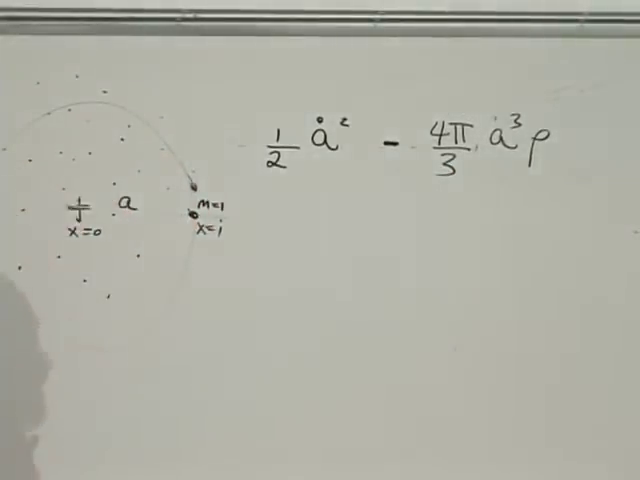
\includegraphics[width=0.78\textwidth]{lecture_03_figure_02.png}
\caption{\(x=0\)을 중심으로 한 균일한 구, \(x=1\)에 있는 공변 은하, 그리고 \(a(t)\)에 대한 뉴턴 역학적 에너지 균형.}
\end{figure}

반지름이 \(a(t)\)인 구 안의 물질만이 \(x=1\)에 있는 입자에 중력을 가한다. 이 입자의 질량을 단위 질량으로 두면 운동 에너지는 다음과 같다.
\begin{equation}
\frac{1}{2}\dot a^2.
\end{equation}
구 안에 포함된 질량은
\begin{equation}
M_{\mathrm{enc}}=\frac{4\pi}{3}a^3\rho,
\end{equation}
이므로 중력 위치 에너지는
\begin{equation}
-\frac{G M_{\mathrm{enc}}}{a}
=
-\frac{4\pi G}{3}a^2\rho.
\end{equation}
\editorialnote{강의 시각 00:05:30에 판에는 운동 항과 밀도에 의존하는 위치 에너지 항이 명확히 적혀 있다. 여기에 적힌 전체 계수는 강의에서 구두로 설명한 유도에 따른다.}

에너지 보존에 따라
\begin{equation}
\frac{1}{2}\dot a^2-\frac{4\pi G}{3}a^2\rho=\text{const}.
\end{equation}
상수는 \(-k\)로 표기한다. 다만 통상적인 정규화에서는 방정식에 \(2\)를 곱한 뒤에야 이 표기가 정해진다는 점에 유의해야 한다. 표준형은
\begin{equation}
\dot a^2=\frac{8\pi G}{3}a^2\rho-k,
\end{equation}
이고, \(a^2\)로 나누면
\begin{equation}
\left(\frac{\dot a}{a}\right)^2=\frac{8\pi G}{3}\rho-\frac{k}{a^2}.
\end{equation}
이 된다. 이것이 여기서 논의하는 동안 사용하는 형태의 프리드만 방정식이다.

\begin{figure}[ht]
\centering
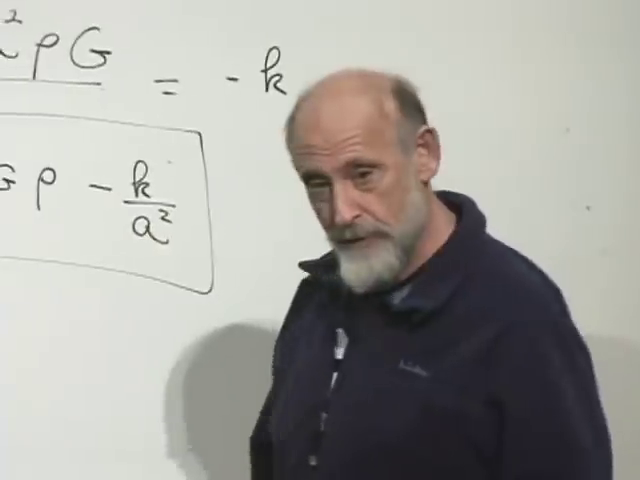
\includegraphics[width=0.56\textwidth]{lecture_03_figure_03.png}
\caption{프리드만 방정식에서 분리해 나타낸 곡률 항 \(-k/a^2\).}
\end{figure}

곡률 항은 관측상 0에 매우 가깝기 때문에, 이 수준에서는 무시해도 아주 좋은 근사가 된다. 이 항은 공간의 곡률에 해당하지만, 관측값이 너무 작아 여기서는 곡률의 부호조차 정할 수 없다.

같은 방정식은 일반 상대성 이론에서도 얻어진다. 시간-시간 성분의 아인슈타인 방정식을 개략적으로 쓰면
\begin{equation}
R_{00}-\frac{1}{2}g_{00}R \propto T_{00}.
\end{equation}
\editorialnote{여기서는 정확한 전체 수치 계수가 아니라 텐서 구조만 제시한다.}
팽창하는 균일한 계량을 쓰면 기하학적 측에서는 \(\dot a/a\)와 \(k/a^2\)의 조합이 나오고, 물질 측에서는 에너지 밀도가 나온다. 이 단계에서는 뉴턴 역학적 논증과 아인슈타인 방정식이 같은 내용을 말한다.

이로 인해 \(\rho\)의 의미도 달라진다. 이제부터는 \(\rho\)를 에너지 밀도라고 부르는 편이 낫다. 공변 좌표계에서 느리게 움직이는 물질의 경우, 이는 곧 정지 에너지 밀도다.

\section{물질 우세 시대}

이제 에너지 밀도가 공변 좌표계에서 정지해 있는 물질에 실려 있다고 가정하자. 한 변이 좌표 단위 길이인 정육면체를 생각한다. 각 변의 물리적 길이는 \(a(t)\)이므로 물리적 부피는 \(a^3(t)\)이다. 이 공변 정육면체 안의 질량-에너지가 \(M\)이고, 물질이 흐름을 따라 움직여 경계를 넘지 않는다면
\begin{equation}
\rho_m=\frac{M}{a^3}.
\end{equation}

이것이 물질 우세 경우다. 이 이상화에서는 입자들이 상자 안에서 정지해 있으므로 온도와 압력을 모두 0으로 둔다. 압력이 있으려면 입자들이 상자의 경계를 통과해야 한다.

\(k\approx 0\)이면 방정식은
\begin{equation}
\left(\frac{\dot a}{a}\right)^2=\frac{8\pi G}{3}\frac{M}{a^3}.
\end{equation}
이 된다. 거듭제곱 꼴을 가정해 보자.
\begin{equation}
a(t)=Ct^p.
\end{equation}
그러면
\begin{equation}
\frac{\dot a}{a}=\frac{p}{t},
\end{equation}
이므로 좌변은 \(t^{-2}\)에 비례하고 우변은 \(t^{-3p}\)에 비례한다. 거듭제곱을 맞추면
\begin{equation}
3p=2,
\qquad
p=\frac{2}{3}.
\end{equation}
을 얻는다. 따라서
\begin{equation}
a(t)\propto t^{2/3}.
\end{equation}
이고, 계수까지 유지하면
\begin{equation}
C^3=6\pi G M.
\end{equation}

해의 핵심은 거듭제곱 법칙이다. 물질이 지배하는 우주는 시간에 선형적으로 비례해 팽창하는 것이 아니라 시간의 3분의 2제곱에 비례해 팽창한다. 이 법칙은 빅뱅 후 대략 \(10^5\)년부터 몇십억 년 뒤까지 이어지는 긴 중간 시대를 설명한다. 현재 우주는 문자 그대로 물질이 지배하는 상태가 아니다. 지금은 암흑 에너지가 지배적이기 때문이다. 그러나 보통 물질과 우주 역사의 상당 기간은 이 법칙으로 설명된다.

\section{복사 우세 시대}

그보다 이른 시기에는 에너지 밀도에서 복사가 우세했다. 이유는 간단하다. 우주에는 엄청난 수의 광자가 있어 양성자 하나당 대략 \(10^9\)개의 광자가 존재하며, 우주가 압축되면 이 광자들의 에너지가 커진다.

광자에는 정지 질량이 없지만 에너지는 있다. 광자의 에너지는
\begin{equation}
E_\gamma=h\nu=\frac{hc}{\lambda}.
\end{equation}
이다. 핵심 가정은 우주가 팽창할 때 광자의 파장도 함께 늘어난다는 것이다.
\begin{equation}
\lambda\propto a.
\end{equation}
상자 안의 파동을 떠올리면 이해하기 쉽다. 상자가 커지면 그 안의 모드의 파장도 상자와 함께 늘어난다. 여기서는 팽창하는 우주에 같은 생각을 적용한다.

\(\lambda\propto a\)이므로 각 광자의 에너지는
\begin{equation}
E_\gamma\propto a^{-1}.
\end{equation}
에 비례한다. 다시 공변 단위 상자를 생각하자. 광자들은 드나들지만, 상자 안의 광자 수는 평균적으로 일정하다. 그러면 상자 안의 전체 광자 에너지도 \(a^{-1}\)에 비례한다. 이를 물리적 부피 \(a^3\)로 나누면 복사 에너지 밀도는
\begin{equation}
\rho_r\propto a^{-4}.
\end{equation}
에 비례한다.

이 추가적인 \(a^{-1}\) 인자가 차이를 만든다. 물질은 우주가 팽창하기 때문에 희석된다. 복사는 그 이유로 희석될 뿐 아니라 각 광자의 적색편이 때문에 에너지도 줄어든다.

따라서 복사 우세 우주에 대한 프리드만 방정식은
\begin{equation}
\left(\frac{\dot a}{a}\right)^2=\frac{8\pi G}{3}\frac{M_r}{a^4}.
\end{equation}
이다. \editorialnote{강의에서는 이 새로운 상수에도 기호 \(M\)를 다시 사용한다. 여기서는 물질의 경우와 혼동하지 않도록 아래 첨자 \(r\)만 덧붙였다.}

같은 시도 함수 \(a(t)=Ct^p\)를 사용하자. 좌변은 다시 \(t^{-2}\)에 비례하고, 우변은 \(t^{-4p}\)에 비례한다. 거듭제곱을 맞추면
\begin{equation}
4p=2,
\qquad
p=\frac{1}{2}.
\end{equation}
을 얻는다. 따라서
\begin{equation}
a(t)\propto t^{1/2}.
\end{equation}
이고, 계수까지 유지하면
\begin{equation}
C^4=\frac{32\pi G}{3}M_r.
\end{equation}

\begin{classroomqa}
\lecturetimestamp{00:35:41}
\audiencequestion{여기에 \(G\)가 들어가는 이유가 뭔가요?}
\lecturerresponse{중력을 만드는 것은 정지 질량만이 아니라 에너지 밀도이기 때문입니다. 느리게 움직이는 물질에서는 그 차이를 알아차리기 어렵지만, 광자를 보면 분명해집니다. 광자는 정지 질량이 없는데도 중력을 만듭니다.}
\end{classroomqa}

복사로 가득 찬 상자를 생각하면 요점이 분명해진다. 광자가 들어 있는 상자를 밀어 보자. 상자가 가속하기 시작하면 광자 쪽으로 움직이는 벽은 광자에게서 멀어지는 벽보다 더 강한 충격을 받으므로, 복사압에 맞서 더 큰 힘으로 밀어야 한다. 따라서 상자는 추가 관성을 갖고, 등가 원리에 따르면 이 추가 관성은 추가 중력 질량도 의미한다. 에너지가 중력을 만든다고 설명할 때 여기서 사용하는 것이 바로 이 광자 상자 논증이다.

\begin{classroomqa}
\lecturetimestamp{00:38:11}
\audiencequestion{시간이 지나면서 감소하는 \(a\)를 갖는 해가 이 방정식들 중 하나라도 있나요?}
\lecturerresponse{있습니다. 곡률 항 \(k/a^2\)을 되살리면 팽창했다가 수축하는 해가 존재합니다. 우리 우주는 그렇게 움직이는 것처럼 보이지 않지만, 방정식은 그런 해를 허용합니다.}
\end{classroomqa}

\begin{classroomqa}
\lecturetimestamp{00:38:44}
\audiencequestion{에너지 보존은 어떻게 된 건가요?}
\lecturerresponse{\(k\) 항을 되살리고 방정식에 다시 \(a^2\)을 곱하면, 우주론 방정식은 정확히 보존 법칙이 됩니다. 한쪽에 있는 물질이나 복사는 장부에 기록되는 항의 일부일 뿐입니다. 팽창은 운동 에너지와 중력 에너지 항을 보태며, 전체 에너지 균형은 보존됩니다.}
\end{classroomqa}

\section{물질과 복사의 공존}

실제 우주론에서는 물질과 복사가 모두 존재한다. 두 성분의 밀도는 서로 다르게 변한다.
\begin{equation}
\rho_m\propto a^{-3},
\qquad
\rho_r\propto a^{-4}.
\end{equation}
따라서 \(a\)가 작을 때는 복사가 우세하고, \(a\)가 클 때는 물질이 우세하다. 시간을 거슬러 올라가면 초기 우주는 복사 우세였음이 틀림없다.

\begin{figure}[ht]
\centering
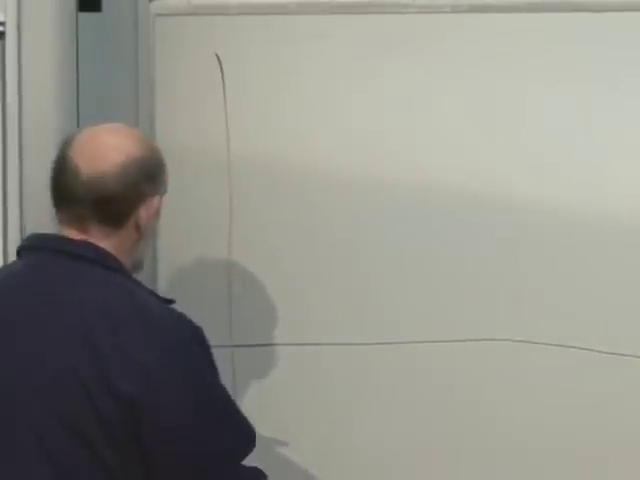
\includegraphics[width=0.68\textwidth]{lecture_03_figure_05.png}
\caption{척도 인자의 함수로서 물질과 복사의 에너지 밀도를 비교하기 위한 축.}
\end{figure}

\editorialnote{강의 시각 00:44:45에 판에는 비교 그래프의 축만 처음으로 나타난다. 바로 뒤에서 논의하는 물질 곡선과 복사 곡선은 다시 그리지 않고 본문에서 설명한다.}

물질 곡선은 \(a^{-3}\)에 따라 감소하고, 복사 곡선은 \(a^{-4}\)에 따라 감소한다. 두 곡선 모두 \(a\to 0\)일 때 발산하지만, 그 지점에서 복사 곡선이 더 빠르게 증가하므로 두 곡선은 등가 척도 인자에서 교차한다. 대략적인 추정에 따르면 이 전이는 약 \(10^4\)년 뒤에 일어나며, 실제로는 조금 더 늦을 수도 있다.

같은 내용을 \(a(t)\)를 \(t\)의 함수로 나타낸 그래프에서도 볼 수 있다. 초기에는 팽창이 \(t^{1/2}\)처럼 진행되고, 나중에는 \(t^{2/3}\)처럼 진행된다. 변화는 갑작스럽게 일어나지 않고, 비교적 좁은 시간 범위에 걸쳐 연속적으로 교차한다.

\begin{classroomqa}
\lecturetimestamp{00:44:04}
\audiencequestion{우주가 나이를 먹으면서 거듭제곱 \(p\)가 \(1/2\)에서 \(2/3\)로 연속적으로 변하나요?}
\lecturerresponse{그렇습니다. 갑자기 바뀌지는 않습니다. 꽤 좁은 시간 범위에서 일어나기는 하지만 변화는 연속적입니다.}
\end{classroomqa}

\section{온도, 재결합, 최종 산란}

다음으로 살펴볼 양은 온도다. 전형적인 광자의 에너지가 \(a^{-1}\)에 비례한다면, 복사 열욕의 온도도 마찬가지다.
\begin{equation}
T\propto a^{-1}.
\end{equation}
\(a\)가 두 배가 되면 온도는 절반으로 낮아진다.

현재 광자 온도를 약 \(3\,\mathrm K\), 이온화 온도를 약 \(3000\,\mathrm K\)로 두자. 후자는 대략 태양 표면의 온도다. 그러면
\begin{equation}
\frac{a_{\mathrm{today}}}{a_{\mathrm{ion}}}\sim 10^3.
\end{equation}
후기 물질 우세 시대의 법칙 \(a\propto t^{2/3}\)을 사용하면
\begin{equation}
\left(\frac{t_{\mathrm{today}}}{t_{\mathrm{ion}}}\right)^{2/3}\sim 10^3,
\end{equation}
이므로
\begin{equation}
\frac{t_{\mathrm{today}}}{t_{\mathrm{ion}}}\sim 1000^{3/2}\sim 3\times 10^4.
\end{equation}
이 추정의 정확도에서 우주의 나이를 \(10^{10}\)년으로 두면
\begin{equation}
t_{\mathrm{ion}}\sim 3\times 10^5\ \mathrm{years}.
\end{equation}

이 시기에 수소와 헬륨은 더 이상 완전히 이온화된 상태를 유지하지 않는다. 그보다 이른 우주는 뜨거운 플라스마다. 플라스마는 왜 불투명할까? 자유 전하가 전자기파에 강하게 반응하기 때문이다. 전기장이 전하를 앞뒤로 움직이고, 매질은 도체처럼 거동하며, 도체는 불투명하다. 이것이 태양 표면과 관련된 비유다.

우주가 충분히 식어 전자가 원자핵과 재결합하면 보통의 중성 원자가 형성되고 우주는 훨씬 투명해진다. 이 전이는 무한히 날카롭지는 않다. 어느 정도 퍼진 구간, 즉 흐릿한 시간 범위에 걸쳐 일어나지만, 우주론에서 다루기에는 충분히 뚜렷하므로 최종 산란면이라고 부른다.

바깥을 본다는 것은 시간을 거슬러 본다는 뜻이다. 가까운 은하에서는 최근 과거를 보고, 더 먼 은하에서는 더 이른 시기를 본다. 충분히 멀리 보면 모든 시선이 우주가 아직 이온화되어 불투명했던 시기에 이른다. 전자기 복사로는 그보다 더 이른 시기를 볼 수 없다.

원리적으로는 다른 메신저 입자들로 더 이른 시기를 탐사할 수 있다. 중성미자는 전기적으로 중성이므로 더 이른 시기에 열적 평형에서 분리되었을 것이다. 중력자는 관측할 수만 있다면 그보다 더 이른 시대에서 왔을 것이다. 그러나 초기 플라스마를 통과하게 해 주는 약한 상호작용 때문에 이 입자들은 검출하기도 매우 어렵다.

우주가 한때 모든 방향에서 태양 표면만큼 뜨거웠다면, 하늘은 왜 눈부시게 밝지 않을까? 최종 산란면이 멀어지고 있고, 거기서 도착하는 광자들이 \(10^3\) 정도의 비율만큼 적색편이되었기 때문이다. 이는 \(3000\,\mathrm K\)와 \(3\,\mathrm K\) 사이의 비율과 대략 같다. 우리에게 도달하는 것은 가시광선이 아니라 마이크로파 복사다.

\begin{classroomqa}
\lecturetimestamp{01:03:51}
\audiencequestion{그러면 우리 망원경으로는 약 \(300{,}000\)년보다 더 이른 시기를 볼 수 없나요?}
\lecturerresponse{전자기파 망원경으로는 볼 수 없습니다. 그 시기 이전의 우주는 이온화되어 불투명했습니다. 원리적으로는 다른 메신저 입자들로 더 이른 시대를 탐사할 수 있습니다.}
\end{classroomqa}

\begin{classroomqa}
\lecturetimestamp{01:08:43}
\audiencequestion{광자의 온도라고 할 때는 그 광자의 최고 복사에 해당하는 흑체의 온도를 뜻하는 거죠. 그런데 그 온도는 파장에 선형적으로 비례하지 않죠?}
\lecturerresponse{맞습니다. 온도는 본질적으로 전형적인 광자의 에너지이므로, 광자의 경우 파장에 반비례합니다. \(T^4\) 법칙은 개별 광자의 에너지가 아니라 에너지 밀도를 가리킵니다. 이 법칙은 광자 하나당 에너지와 단위 부피당 광자 수를 결합하며, 수밀도는 \(T^3\)에 비례합니다.}
\end{classroomqa}

따라서
\begin{equation}
n_\gamma\propto T^3,
\qquad
\rho_\gamma\propto T^4.
\end{equation}

\section{회전 곡선으로 알아보는 암흑 물질}

암흑 물질은 은하 회전 곡선을 통해 등장한다. 이는 대규모 프리드만 방정식에서 추론된 것이 아니라 은하 규모의 천문 관측에서 추론되었다.

가장 단순한 뉴턴 역학 문제부터 시작하자. 질량 \(m\)인 가벼운 물체가 중심 질량 \(M\)을 반지름 \(r\)인 궤도로 돈다고 하자. 중력은
\begin{equation}
\frac{GMm}{r^2},
\end{equation}
이고 구심 가속도는 \(v^2/r\)이다. 뉴턴 법칙에 따르면
\begin{equation}
m\frac{v^2}{r}=\frac{GMm}{r^2}.
\end{equation}
이다. \(m\)를 약분하고 \(r\)를 곱하면
\begin{equation}
v(r)=\sqrt{\frac{GM}{r}}.
\end{equation}
을 얻는다. 따라서 중력을 만드는 질량이 중심 부근에 집중되어 있다면 공전 속도는 \(r^{-1/2}\)에 따라 감소한다.

질량이 빛을 따라 분포한다면 이렇게 예상할 수 있다. 은하에서 보이는 물질 대부분은 중심핵 부근에 있으므로 바깥쪽 별들은 태양계 바깥 행성들과 비슷하게 움직일 것이다. 천문학자들은 가까운 은하의 양쪽에서 도플러 편이 차이를 측정해 공전 속도를 추론한다. 이때 은하 전체의 후퇴 운동을 먼저 빼고, 우리 쪽으로 다가오는 쪽과 멀어지는 쪽을 비교한다. 측정된 공전 속도는 큰 반지름까지 대체로 일정하게 유지된다.

그러므로 중심 질량 \(M\) 대신 반지름 안에 포함된 질량 \(M(r)\)를 넣으면
\begin{equation}
\frac{v^2}{r}=\frac{G M(r)}{r^2}.
\end{equation}
이 된다. \(v(r)\)가 대략 일정하다면
\begin{equation}
M(r)\propto r.
\end{equation}
이다. 다시 말해, 보이는 빛이 더는 증가하지 않는 곳에서도 중력을 만드는 질량은 반지름에 따라 계속 증가한다.

이제 논의에서 단순화를 위해 가정하듯 질량 분포가 대략 구형이라고 하자. 그러면
\begin{equation}
M(R)=\int_0^R 4\pi r^2\rho(r)\,dr.
\end{equation}
이다. \(M(R)\propto R\)라면 \(R\)에 대해 미분하여
\begin{equation}
4\pi R^2\rho(R)\propto 1,
\end{equation}
을 얻으며, 따라서
\begin{equation}
\rho(r)\propto \frac{1}{r^2}.
\end{equation}

\begin{classroomqa}
\lecturetimestamp{01:28:18}
\audiencequestion{밀도가 \(1/r^2\)에 비례할 것 같은데, 그 이유가 있나요?}
\lecturerresponse{관측된 평탄한 회전 곡선으로부터 \(M(R)\propto R\)를 추론하고, 이를 미분하면 \(\rho(r)\propto 1/r^2\)을 얻습니다. 그 이상으로는 여기서 간단한 제일 원리 설명을 주장하지 않습니다. 상세한 시뮬레이션이 많은 부분을 담당합니다.}
\end{classroomqa}

확실한 결론은 은하에 발광 물질만으로 예상되는 것보다 훨씬 많은 중력 질량이 있다는 점이다. 그 질량은 몇 배가량 더 많으며, 여기서 사용한 추정치로는 대략 한 자릿수 정도 더 많다. 보이는 은하는 훨씬 큰 암흑 헤일로 안에 놓여 있다.

보통의 기체는 어떻게 그렇게 희박한 상태에 머무르지 않을까? 소산 때문이다. 충돌과 마찰 같은 과정, 그리고 복사로 에너지를 잃을 수 있기 때문에 기체 구름은 수축한다. 암흑 물질은 유의미한 복사를 하지 않고 거의 충돌하지 않는 것으로 보인다. 중력은 암흑 물질을 안쪽으로 끌어당겨 위치 에너지를 운동 에너지로 바꿀 수 있지만, 효율적인 소산이 없으면 보통 물질이 만드는 작고 밝은 구조로 붕괴하지 않는다. 헤일로를 확장된 상태로 유지하는 것은 운동 에너지다.

이어서 몇 가지 대안이 신중하게 논의된다. 중성미자는 은하 규모에서 이런 식으로 거동하기에는 너무 빠르다고 한다. 보통의 수소로 이루어진 헤일로는 초기 우주의 핵합성을 크게 교란할 것이다. 보통의 물질로 이루어진 블랙홀도 문제가 될 수 있다고 언급한다. 초기 우주에 보통 물질이 너무 많다는 뜻이 되고 중력 렌즈 효과와 관련된 문제도 일으킬 수 있기 때문이다. 강의에서는 그 자리에서 이 이상의 주장을 하지는 않는다.

헤일로는 얇은 껍질이나 토러스 형태로 묘사되지 않는다. 중심부가 더 조밀하고 바깥쪽으로 갈수록 점진적으로 희박해지는, 대략 구형의 불균일한 덩어리다.

\begin{classroomqa}
\lecturetimestamp{01:53:12}
\audiencequestion{불릿 성단을 말씀하시는 건가요?}
\lecturerresponse{그렇습니다. X선 기체는 보통 물질을 보여 주고, 중력 렌즈 효과는 중력을 만드는 전체 질량을 보여 줍니다. 충돌 과정에서 두 분포는 서로 분리됩니다. 이는 보이는 물질에만 작용하는 단순한 중력 수정이 아니라 실제 암흑 물질이 존재한다는 강력한 증거입니다.}
\end{classroomqa}

이것이 마지막 관측상의 요점이다. 암흑 물질이 무엇인지에 관해 구체적으로 알려진 것은 거의 없지만, 여기서 급진적인 새 원리를 가정할 필요는 없다. 보수적으로 생각하면 자연에는 아직 확인되지 않은, 약하게 상호작용하는 입자들이 추가로 존재한다고 보면 된다.
